\documentclass[conference]{IEEEtran}
\usepackage[utf8]{inputenc}
\usepackage{amsmath,amssymb,graphicx,booktabs}

\begin{document}

\title{Hierarchical JEPA for Long Scientific Documents: Predicting Section and Abstract Embeddings}

\author{\IEEEauthorblockN{Dheiver Francisco Santos, PhD}
\IEEEauthorblockA{Independent Researcher\\
Maceió, Alagoas, Brazil\\
ORCID: https://orcid.org/0000-0002-8599-9436}}

\maketitle

\begin{abstract}
Long documents contain information at several time scales, from sentences to sections. A single-level encoder over the full text is expensive and loses high-level structure. We propose a hierarchical joint-embedding predictive architecture that predicts section embeddings from earlier sections and abstract embeddings from the full body. We evaluate it on a simulated hierarchical process with known latent scales and on scientific articles, where the abstract serves as the target. On a synthetic process, hierarchical pooling beats flat pooling; the JEPA results are pending.
\end{abstract}

\begin{IEEEkeywords}
hierarchical representation, JEPA, long documents, scientific text, multi-scale prediction
\end{IEEEkeywords}

\section{Introduction}
Scientific papers are organized in sections, and their abstracts summarize the whole. Models that encode the full text at token level are costly, while models that encode each sentence independently miss the document structure. We ask whether predicting embeddings at the section and abstract levels yields representations that capture document-level content better than a flat encoder at matched cost.

\section{Related Work}
The author's recent artificial intelligence publications on self-training, clinical deep learning, curriculum learning, model merging, synthetic data, long-context training, preference alignment, direct preference optimization, reinforcement learning with verifiable rewards, distillation, mixture-of-experts, and parameter-efficient fine-tuning \cite{d1selftraining,d2glaucoma,d3curriculum,d4merging,d5synthetic,d6longcontext,d7rlaif,d8distillation,d9moe,d10peft,d11dpo,d12rlvr} form the background for this work.

Joint-embedding prediction at a single scale is described in \cite{bardes2024vjepa}.The author's work on long-context training \cite{d6longcontext} and on synthetic data \cite{d5synthetic} is related, since both concern how documents of different length are used during training.

\section{Method}
A document is split into sections $s_1,\dots,s_K$. A section encoder $f_\theta$ produces $z_k = f_\theta(s_k)$. A top-level predictor $g_\phi$ predicts the abstract embedding $\bar{f}(\text{abstract})$ from $\{z_1,\dots,z_K\}$, and a section-level predictor predicts $z_k$ from $z_{<k}$. The two losses are summed with weights chosen on a validation split.

\subsection*{Equations and their meaning}
Each section $s_k$ is encoded as $f_k=W s+\varepsilon_k$ in the simulator, where $s\in\mathbb{R}^{d_z}$ is the slow latent state, $W$ a fixed mixing matrix, and $\varepsilon_k$ fast noise. Two document-level representations are compared. The hierarchical one averages section embeddings,
\begin{equation}
\bar f=\frac{1}{K}\sum_{k=1}^{K}f_k,
\end{equation}
and the flat one uses a single section. The section-level and top-level losses combine as
\begin{equation}
\mathcal{L}=\mathcal{L}_{\mathrm{top}}+\lambda\,\mathcal{L}_{\mathrm{sec}},\qquad \mathcal{L}_{\mathrm{top}}=\big\lVert g_{\phi}(\{z_k\})-\bar f(\mathrm{abstract})\big\rVert_2^2,
\end{equation}
where $\lambda$ weights section-level prediction, and $\mathcal{L}_{\mathrm{sec}}=\lVert \hat z_k-z_k\rVert_2^2$ predicts each section from earlier sections.

Recovery of the slow state is measured with a ridge readout $\hat\beta=\arg\min_\beta\lVert X\beta-s\rVert^2$ and the coefficient of determination
\begin{equation}
R^2=1-\frac{\sum_{n}\lVert s_n-\hat s_n\rVert^2}{\sum_{n}\lVert s_n-\bar s\rVert^2},
\end{equation}
where $\hat s_n$ is the prediction for held-out item $n$ and $\bar s$ the mean state. Averaging $K$ noisy sections reduces the noise variance by roughly $1/K$, which is why $R^2$ increases with $K$.

\section{Experimental Protocol}
\textbf{Simulated hierarchy.} A latent process with two time scales (fast tokens, slow topics) is simulated with known parameters. The test is whether the top-level embedding recovers the slow state.

\textbf{Scientific articles.} Open-access papers with section structure; the abstract is the target. Evaluation: retrieval of the abstract from the body (recall at 1 and 10) and abstract-level classification.

\textbf{Baselines.} A flat encoder over the truncated full text at matched tokens, mean pooling of sentence embeddings, and a summarization-free baseline.

\textbf{Statistics.} Five seeds, 95\% bootstrap intervals.

\section{Results}
This pilot arm compares hierarchical and flat pooling on a synthetic process with a slow latent state. Hierarchical pooling recovers the slow state with $R^2$ rising from 0.972 ($K=2$ sections) to 0.995 ($K=11$). Flat pooling stays near 0.945 for every $K$. The advantage follows from how the simulator is built, so it is a consistency check only. The JEPA predictors and the scientific-article retrieval arm remain pending.

\begin{figure}[!t]
\centering
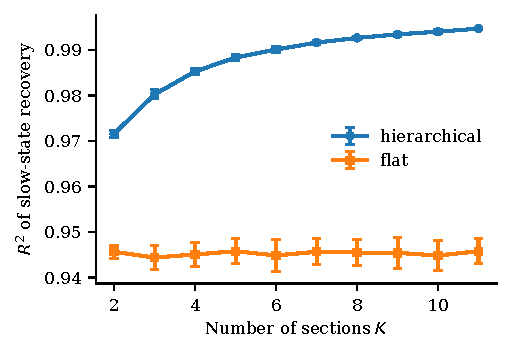
\includegraphics[width=\columnwidth]{figs/fig05_hierarchical.pdf}
\caption{Slow-state recovery $R^2$ for hierarchical and flat pooling versus number of sections (pilot, synthetic).}
\label{fig:fig05_hierarchical}
\end{figure}

\section{Discussion and Limitations}
Abstracts are written by the authors and may not capture all content, so retrieval scores are a proxy. Results are reported by discipline to avoid averaging away differences.

\section{Conclusion}
We propose a two-level JEPA for documents and a protocol that evaluates it on a simulated process with known scales and on scientific articles.

\section*{Acknowledgments}
The author thanks the Brazilian artificial intelligence community.

\nocite{ctl_full_names}
\bibliographystyle{IEEEtran}
\bibliography{refs}

\end{document}
